\section[Адаптивная сеть на основе системы нечеткого вывода]{%
  АДАПТИВНАЯ СЕТЬ НА ОСНОВЕ СИСТЕМЫ НЕЧЕТКОГО ВЫВОДА
}

Под \emph{нейронными сетями} подразумеваются вычислительные структуры,
которые моделируют простые биологические процессы,
обычно ассоциируемые с процессами человеческого мозга.
Элементарным преобразователем в данных сетях является \emph{искусственный нейрон}
или просто нейрон, названный так по аналогии с биологическим прототипом~\cite{kruglov2001}.

На рисунке~\ref{fig:struct_neuron} показана структура искусственного нейрона.
В соответствии с ней, в состав нейрона входят умножители (синапсы),
сумматор и нелинейный преобразователь.

\begin{figure}[h!]
  \centering
  \fcolorbox{gray}{white}{
    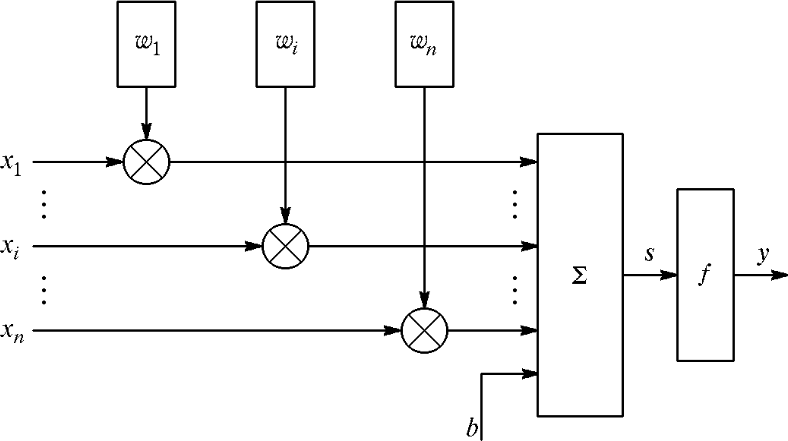
\includegraphics[width=120mm]{fig/struct_neuron}
  }
  \caption{Структура искусственного нейрона}
  \label{fig:struct_neuron}
\end{figure}

\emph{Синапсы} осуществляют связь между нейронами и умножают входной сигнал на число,
характеризующее силу связи, --- вес синапса.
\emph{Сумматор} выпроняет сложение сигналов, поступающих по синаптическим связям от
других нейронов и внешних входных сигналов.
\emph{Нелинейный преобразователь} реализует нелинейную функцию одного аргумента,
называемую \emph{функцией активации}.
Одной из наиболее распространенных функций активации является
так называемая \emph{логистическая функция}, или сигмоид
\[
  f(s) = \dfrac{1}{1 + e^{-as}}.
\]

В процессе функционирования нейросети можно выделить два этапа:
\begin{enumerate}
\item Обучение, в ходе которого производится настройка сети на основании
  учебных примеров исходных данных, носящих репрезентативный характер.
\item Применение, в ходе которого осуществляется решение
  поставленной задачи классификации, прогнозирования, управления и~т.~п.
  на основании реальных исходных данных.
\end{enumerate}

Теоретически, системы с нечеткой логикой и искусственные нейросети эквивалентны
друг другу, однако на практике у них имеются свои собственные достоинства и недостатки.
Например, нейронные сети хороши для задач распознавания образов, но весьма неудобны
для выяснения вопроса, как они подобное распознавание осуществляют.
Они могут приобретать знания, но процесс их обучения зачастую происходит достаточно
медленно, а анализ обученной информации весьма сложен.
При этом ввести в нейронную сеть какую-либо априорную информацию для ускорения
её обучения невозможно.
Системы с нечеткой логикой, напротив, хороши для объяснения получаемых с их
помощью выводов, но они не могут автоматически приобретать знания для использования
их в механизмах выводов.
Подобные соображения легли в основу аппарата гибридных сетей,
способных не только использовать априорную информацию,
но и приобретать новые знания, оставаясь при этом логически прозрачными для пользователя.

\emph{Гибридная нейронная сеть} --- это нейронная сеть с четкими сигналами,
весами и активационной функцией, использующая для объединения сигналов
t-норму или t-конорму.

Рассмотрим примеры элементарных гибридных сетей.
\begin{enumerate}
\item Нечеткий нейрон <<И>>.
  В данном случае сигналы \( x_i \) и веса \( w_i \) объединяются с помощью t-конормы:
  \( p_i = S(w_i, x_i), \: i = 1, 2, \)
  а выход образуется с применением t-нормы:
  \( y = T(p_1, p_2) = T(S(w_1, x_1), S(w_2, x_2)), \)
  как показано на рисунке~\ref{fig:hybrid_and}.

  \begin{figure}[h!]
    \centering
    \fcolorbox{gray}{white}{
      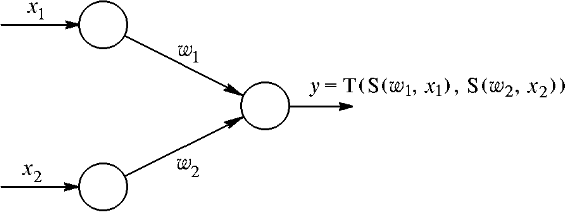
\includegraphics[width=92mm]{fig/hybrid_and}
    }
    \caption{Структура гибридного нейрона <<И>>}
    \label{fig:hybrid_and}
  \end{figure}

\item Нечеткий нейрон <<ИЛИ>>.
  В данном случае сигналы \( x_i \) и веса \( w_i \) объединяются с помощью t-нормы:
  \( p_i = T(w_i, x_i), \: i = 1, 2, \)
  а выход образуется с применением t-нормы:
  \( y = S(p_1, p_2) = S(T(w_1, x_1), T(w_2, x_2)), \)
  как показано на рисунке~\ref{fig:hybrid_or}.

  \begin{figure}[h!]
    \centering
    \fcolorbox{gray}{white}{
      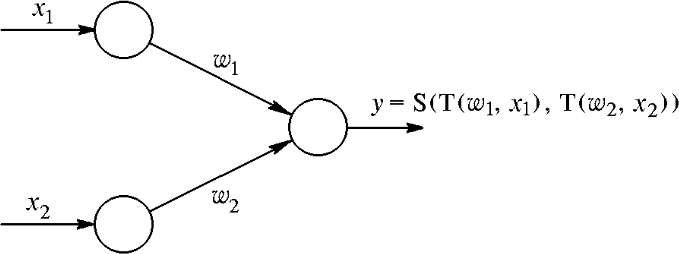
\includegraphics[width=92mm]{fig/hybrid_or}
    }
    \caption{Структура гибридного нейрона <<ИЛИ>>}
    \label{fig:hybrid_or}
  \end{figure}
\end{enumerate}

Для осуществления нечеткого логического вывода
гибридные нейроны объединяются в сеть, как показано на рисунке~\ref{fig:anfis}.
В зарубежной литературе приведенная архитектура носит название ANFIS
(от англ. Adaptive Neuro-Fuzzy Inference System).

\begin{figure}[h!]
  \centering
  \fcolorbox{gray}{white}{
    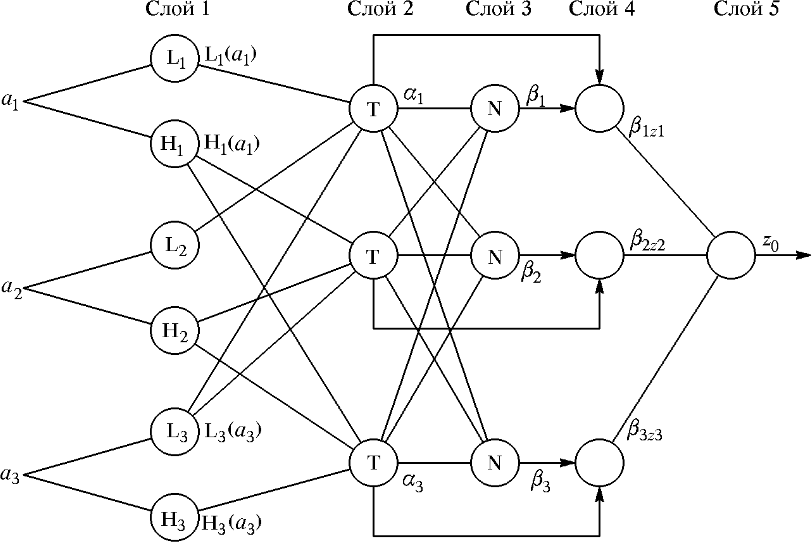
\includegraphics[width=120mm]{fig/anfis}
  }
  \caption{Структура гибридной нейронной сети \\ (архитектура ANFIS)}
  \label{fig:anfis}
\end{figure}

Рассмотрим структуру данной сети, принимая во внимание, что она соответствует
следующему набору правил: \par
\( \text{П}_1 \): если
\( x_1 \) есть \( L_1 \) и
\( x_2 \) есть \( L_2 \) и
\( x_3 \) есть \( L_3 \),
то \( y \) есть \( H \), \par
\( \text{П}_2 \): если
\( x_1 \) есть \( H_1 \) и
\( x_2 \) есть \( H_2 \) и
\( x_3 \) есть \( L_3 \),
то \( y \) есть \( M \), \par
\( \text{П}_3 \): если
\( x_1 \) есть \( H_1 \) и
\( x_2 \) есть \( H_2 \) и
\( x_3 \) есть \( H_3 \),
то \( y \) есть \( S \).

Выходы узлов первого слоя представляют собой значения функции
принадлежности при заданных значениях входов.
Выходы второго слоя соответствуют значениям истинности условной части
каждого правила вывода, вычисляемые по формулам:
\[
  \begin{aligned}
    \alpha_1 &= L_1(a(1)) \cap L_2(a_2) \cap L_3(a_3), \\
    \alpha_2 &= H_1(a(1)) \cap H_2(a_2) \cap L_3(a_3), \\
    \alpha_3 &= H_1(a(1)) \cap H_2(a_2) \cap H_3(a_3).
  \end{aligned}
\]
Все нейроны данного слоя обозначены буквой T, что означает,
что для осуществления вычислений они могут использовать
произвольную t-норму.
Нейроны, обозначенные буквой N, вычисляют следующие величины:
\[
  \beta_1 = \dfrac{\alpha_1}{\alpha_1 + \alpha_2 + \alpha_3}, \:
  \beta_2 = \dfrac{\alpha_2}{\alpha_1 + \alpha_2 + \alpha_3}, \:
  \beta_3 = \dfrac{\alpha_3}{\alpha_1 + \alpha_2 + \alpha_3}.
\]
Нейроны четвертого слоя выполняют операции:
\[
  \beta_{z_1} = \dfrac{\beta_1}{H(\alpha_1)}, \:
  \beta_{z_2} = \dfrac{\beta_2}{M(\alpha_2)}, \:
  \beta_{z_3} = \dfrac{\beta_3}{S(\alpha_3)}.
\]
Нейрон пятого слоя вычисляет выход сети:
\( z_0 = \beta_{z_1} + \beta_{z_2} + \beta_{z_3}. \)

Для коррекции параметров сети используется может использоваться
метод обратного распространения ошибки, имеющий следующий вид:
\begin{enumerate}
\item Весам сети присваиваются некоторые начальные значения.
\item Выбирается очередная обучающая пара
  \( (A, Z) = ((\alpha_1, \alpha_2, \alpha_3), (z)) \)
  из обучающего множества; вектор \( A \) подается на вход сети.
\item Вычисляется выход сети \( Z_0 = (z_0) \).
\item Вычисляется разность между требуемым (целевым, \( Z \))
  и реальным (вычисленным, \( Z_0 \)) выходом сети.
\item Параметры характеристических функций множеств \( H, M, S \)
  корректируются так, чтобы минимизировать ошибку.
\item Шаги 2--5 повторяются для каждой пары обучающего множества до тех пор,
  пока ошибка на всем множестве не достигнет приемлемой величины.
\end{enumerate}
